%In this section we summarize the results of the experiments described in Section~\ref{ss:exp}.
% LW: I believe all the experiments were done with 3 risk groups- -but all results were shown just
%     for high and low --- what happened to the middle group?
%     It is mentioned so less at the end – the reader may almost interpret as if
%     there were just two risk groups in ur whole experiment.
% JK: I agree, this was confusing, and mostly done to simplify interpretation of the results.
%     I've added back the middle group throughout below, to avoid this confusion,
%     though I don't think this usually adds much to the results.
% ==================================================================================================
\subsection{Experiment 1: The mechanisms by which turnover influences equilibrium incidence and prevalence}  %make sure to use same headings in the Methods
\label{ss:res-prev-inc}
Figure~\ref{fig:1d-prevalence} illustrates trends in equilibrium STI prevalence  
among the high, medium, low, risk groups, at different rates of turnover when controlled by duration 
of time spent in the highest risk group.
In all three groups, there was an inverted U-shaped relationship between STI prevalence and turnover.
Equilibrium prevalence of the STI rose with faster turnover (region~A),
reached a maximum, and then fell at the highest rates of turnover (region~B). %did not understand what is meant by 'cases'? - the three groups or different levels of turnover? use same terms and make sure that the terms (e.g. cases) are defined/easy to know what we are talking about... for consistency and clarity. 
%was hard to follow the sentence. tried to simplify language.
The threshold turnover rate at which group-specific prevalence peaked (i.e. the 
turnover-prevalence relationship transitioned from 
positive to inverse) varied by risk group. 
The high risk group had the lowest turnover threshold (Figure~\ref{fig:1d-prevalence-high}) .
			%what does 'this transition' refer to? first define transition, then say 'the transition' or 'this transition' once the term 'transition' is clearly defined :). 
			% I found the paragraph challenging to follow and had to read and re-read a few times. Tried to edit to simplify the language but might still need some more work.
This inverse U-shaped relationship and turnover threshold can be explained by the interaction between two factors:		%Using a lot of 'this' and 'these'. can we reduce and point to the subject of the sentence specifically? 
%SM: Is 'peaked prevalence profile' an established way to describing or labelling the phenomena? I have never heard of it before, so if yes - please cite. Otherwise, suggest using more commonly used terms for the phenomena, such as U-shaped, non-linear, or concave up / concave down, etc. Try to avoid inventing new terms that are unfamiliar to readers - makes it challenging to read. Only invent when that one single new terminology is the entire focus of the paper.
the movement of individuals between risk groups, and
incidence.												%I like how you set up the explanation before diving into the next section.
\begin{figure}[!tbp]										%Figure 4: y-axis - indicate STI prevalence/incidence (not just prevalence); 
% SM: was unclear why "high-risk" capitalized in Y-label but not in rest of the manuscript? Consistency check and usually the same capitalization approach for axis labels in scientific papers.  
  \centering
  \begin{subfigure}{0.31\linewidth}
    \centering
    \includegraphics[width=\linewidth]{{1d-prevalence-high-tau=0.1}.pdf}
    \caption{High risk}
    \label{fig:1d-prevalence-high}
  \end{subfigure}
  \begin{subfigure}{0.31\linewidth}
    \centering
    \includegraphics[width=\linewidth]{{1d-prevalence-med-tau=0.1}.pdf}
    \caption{Medium risk}
    \label{fig:1d-prevalence-med}
  \end{subfigure}
  \begin{subfigure}{0.31\linewidth}
    \centering
    \includegraphics[width=\linewidth]{{1d-prevalence-low-tau=0.1}.pdf}
    \caption{Low risk}
    \label{fig:1d-prevalence-low}
  \end{subfigure}
  \caption{Equilibrium prevalence among high, medium, and low risk groups
    versus turnover, as controlled by the duration in the high risk group $\delta_H$.
    Turnover shown in log scale.}
  \label{fig:1d-prevalence}
\end{figure}
% --------------------------------------------------------------------------------------------------
\subsubsection{Movement of individuals between risk groups}
The first factor, movement of individuals between risk groups,
is illustrated in Figure~\ref{fig:flows} for four rates of turnover.
We assumed that the distribution of health states among individuals leaving a risk group
is equal to the distribution of health states within the group.
Therefore, in the low risk group,
a higher proportion of individuals leaving the group due to turnover were susceptible,
as compared to individuals entering the group, who were more likely to be infectious.
Thus, in the low risk group,
turnover yielded a net replacement of susceptible individuals with infectious individuals.
As a result, increasing turnover at low rates of turnover
increased prevalence among the low risk group
(Figure~\ref{fig:1d-prevalence-low}, region~A).
Among the high risk group,
turnover yielded a net replacement of both infectious and treated individuals
with susceptible individuals.
However, since incidence in the group was high,
infection of new susceptible individuals from turnover
outpaced the loss of infectious individuals via turnover
for low rates of turnover.
As a result, STI prevalence in the high risk group
also increased with turnover for low rates of turnover
(Figure~\ref{fig:1d-prevalence-high}, region~A).
In order to explain the reversal of these trends in region~B,
the second factor, incidence, must be considered.
\par
\begin{figure}[!tbp]
  \centering
  \begin{subfigure}[t]{0.6\linewidth}
    \centering
    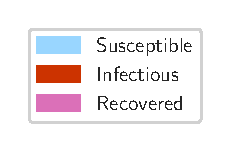
\includegraphics[width=\linewidth]{flows-legend.pdf}
  \end{subfigure}
  \begin{subfigure}[t]{0.15\linewidth}
    \centering
    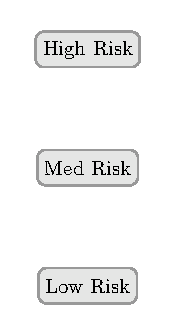
\includegraphics[width=\linewidth]{flows-labels.pdf}
  \end{subfigure}%
  \begin{subfigure}[t]{0.2\linewidth}
    \centering
    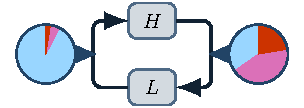
\includegraphics[width=\linewidth]{flows-low.pdf}
    \caption{Low turnover}
    \label{fig:flows-low}
  \end{subfigure}%
  \begin{subfigure}[t]{0.2\linewidth}
    \centering
    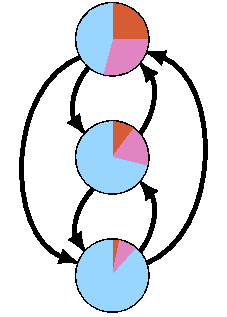
\includegraphics[width=\linewidth]{flows-med.pdf}
    \caption{Moderate turnover}
    \label{fig:flows-med}
  \end{subfigure}%
  \begin{subfigure}[t]{0.2\linewidth}
    \centering
    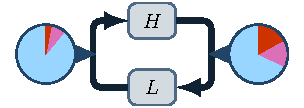
\includegraphics[width=\linewidth]{flows-high.pdf}
    \caption{High turnover}
    \label{fig:flows-high}
  \end{subfigure}%
  \begin{subfigure}[t]{0.2\linewidth}
    \centering
    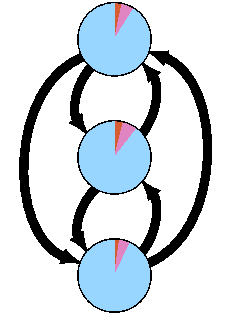
\includegraphics[width=\linewidth]{flows-extreme.pdf}
    \caption{Very high turnover}
    \label{fig:flows-extreme}
  \end{subfigure}
  \caption{Average health states of individuals
    moving between high and low risk groups due to different rates of turnover.}
  \label{fig:flows}
\end{figure}
% --------------------------------------------------------------------------------------------------
\subsubsection{Incidence}
% Next, we examined the second factor in
% the influence of turnover on infection prevalence: incidence.
As shown in Appendix~\ref{aa:eqs-incidence}, incidence
is proportional to two dynamic components:
$\hat{C}_{\mathcal{I}}$ the average contact rate among infectious individuals, and
$\hat{\mathcal{I}}$ overall prevalence.%
\footnote{Since we assumed proportionate mixing among risk groups,
  and only consider heterogeneity in contact rate $C_i$,
  incidence in each risk group is proportional to overall incidence
  with $C_i$ as a scale factor (Figure~\ref{fig:1d-incidence}).}
Therefore, the influence of turnover on equilibrium incidence
can be understood through the influence of turnover on these two components
(Figure~\ref{fig:1d-incidence-factors}).
Increasing turnover monotonically decreased the first component:
$\hat{C}_{\mathcal{I}}$ the average contact rate among infectious individuals
(Figure~\ref{fig:1d-C-I}), because
turnover caused a net movement of infectious individuals from high to low risk.
For low rates of turnover, however,
turnover increased the second component:
$\hat{\mathcal{I}}$ overall prevalence
(Figure~\ref{fig:1d-prev-all}, region~A).
For low rates of turnover,
overall prevalence $\hat{\mathcal{I}}$
increased faster with turnover than
the average contact rate of infectious people $\hat{C}_{\mathcal{I}}$ decreased.
As a product of these two components,
incidence then increased with turnover in region~A
(Figure~\ref{fig:1d-incidence-all}).
The transition between regions~A~and~B in Figure~\ref{fig:1d-incidence-all}
(maximum equilibrium incidence) occurred when the dominating component
between $\hat{\mathcal{I}}$ and $\hat{C}_{\mathcal{I}}$ reversed
% SB: It may be common to write like this in the modeling world,
%     but less so in traditional scientific writing.
%     Ie, normally results would be laid out in an agnostic way
%     and then discussions really provides the interpretation of
%     why this was or was not expected.
%     And the editorializing “therefore” would not be there as much...
% JK: I think it is reasonable to argue that this conclusion is
%     a result, rather than an interpretation, since we've hopefully shown
%     it with the figures directly. I think you're right that this is a
%     modelling thing, but its part of our "results" showing the mechanisms.
-- that is, when
the average contact rate of infectious people $\hat{C}_{\mathcal{I}}$
decreased with turnover faster than prevalence $\hat{\mathcal{I}}$
increased with turnover,
causing incidence to decline.
Then, as rates of turnover increased further,
declining incidence also reduced prevalence,
and incidence and prevalence decreased across all groups
in mutually reinforcing decline.
This mechanism explains the observations shown in region~B throughout.
\begin{figure}[!tbp]
  \centering
  \begin{subfigure}[t]{0.31\linewidth}
    \centering
    \includegraphics[width=\linewidth]{{1d-C-I-tau=0.1}.pdf}
    \caption{Average contact rate among infectious individuals $\hat{C}_{\mathcal{I}}$}
    \label{fig:1d-C-I}
  \end{subfigure}
  \begin{subfigure}[t]{0.31\linewidth}
    \centering
    \includegraphics[width=\linewidth]{{1d-prevalence-all-tau=0.1}.pdf}
    \caption{Overall prevalence $\hat{\mathcal{I}}$}
    \label{fig:1d-prev-all}
  \end{subfigure}
  \begin{subfigure}[t]{0.31\linewidth}
    \centering
    \includegraphics[width=\linewidth]{{1d-incidence-all-tau=0.1}.pdf}
    \caption{Overall incidence $\lambda$}
    \label{fig:1d-incidence-all}
  \end{subfigure}
  \caption{Incidence and the dynamic factors of incidence versus turnover.
    The product of components (\subref{fig:1d-C-I}) and (\subref{fig:1d-prev-all})
    is proportional to (\subref{fig:1d-incidence-all}) overall incidence.}
  \label{fig:1d-incidence-factors}
\end{figure}
% --------------------------------------------------------------------------------------------------
\subsubsection{Prevalence ratios}
Figure~\ref{fig:1d-ratio-prevalence} shows
the equilibrium prevalence ratios in comparisons of all three risk groups.
The prevalence ratio between highest and lowest risk groups
monotonically decreases with turnover
(Figure~\ref{fig:1d-ratio-prevalence-high-low}).
Since incidence ratios were not affected by turnover
(Figure~\ref{fig:1d-ratio-incidence}),
this decrease in prevalence ratio with turnover
was attributed to the movement of individuals between risk groups,
namely infectious individuals from high-to-low risk,
and non-infectious individuals from low-to-high risk.
This movement of individuals can also explain why
prevalence among the high risk group can decrease with turnover,
even as incidence increases
(region~B in Figure~\ref{fig:1d-prevalence-high} overlaps
region~A in Figure~\ref{fig:1d-incidence-all}),
while prevalence among the low risk group can increase with turnover,
even as incidence decreases
(region~A in Figure~\ref{fig:1d-prevalence-low} overlaps
region~B in Figure~\ref{fig:1d-incidence-all}).
The high-to-medium and medium-to-low prevalence ratios are not monotonic,
but for moderate rates of turnover,
they follow the same trends as
the high-to-low prevalence ratio.
% JK: This is tricky to explain and not much value added.
%     Do you think we could cut the para here
%     and omit the next two sentences?
For low rates of turnover, the high-to-medium prevalence ratio
(Figure~\ref{fig:1d-ratio-prevalence-high-med})
increases slightly as prevalence among the high risk group
increases with turnover faster than among the medium risk group.
Similarly, for high rates of turnover, the medium-to-low prevalence ratio
(Figure~\ref{fig:1d-ratio-prevalence-med-low})
increases slightly as prevalence among the medium risk group
declines faster with turnover than among the low risk group.
\begin{figure}
  \centering
  \begin{subfigure}{0.31\linewidth}
    \centering\includegraphics[width=\linewidth]{{1d-ratio-prevalence-high-low-tau=0.1}.pdf}
    \caption{High vs Low risk}
    \label{fig:1d-ratio-prevalence-high-low}
  \end{subfigure}
  \begin{subfigure}{0.31\linewidth}
    \centering\includegraphics[width=\linewidth]{{1d-ratio-prevalence-high-med-tau=0.1}.pdf}
    \caption{High vs Medium Risk}
    \label{fig:1d-ratio-prevalence-high-med}
  \end{subfigure}
  \begin{subfigure}{0.31\linewidth}
    \centering\includegraphics[width=\linewidth]{{1d-ratio-prevalence-med-low-tau=0.1}.pdf}
    \caption{Medium vs Low Risk}
    \label{fig:1d-ratio-prevalence-med-low}
  \end{subfigure}
  \caption{Equilibrium prevalence ratios between risk groups
    under different rates of turnover $\phi$.}
  \label{fig:1d-ratio-prevalence}
\end{figure}
% ==================================================================================================
\subsection{Experiment 2: Inferred risk heterogeneity with vs without turnover}
% SB: I really feel like a separate paper... just a lot of info here!!
% LW: Refresh the readers on under what values of treatment rate and turnover rate did u
%     conduct these experiments.
% JK: @LW done, and @SB hopefully we are much more consise and connected with our story now!
\label{ss:res-infer}
Next, we compared the fitted parameters in models with versus without turnover
($\delta_H = 5$ vs.\ $\delta_H = 33$ years).
Before model fitting, the predicted prevalence ratio
between high and low risk groups was lower with turnover than without:
$\input{\datapath/values/turnover-prevalence-ratio-high-low.txt}$~vs~%
$\input{\datapath/values/no-turnover-prevalence-ratio-high-low.txt}$.
This reflects the ``homogenizing'' effect of turnover on
the average risk experienced by individuals in the model.
As shown in Figure~\ref{fig:1d-ratio-prevalence-high-low},
the high-to-low prevalence ratio consistently declined with turnover.
Thus, when fitting the model to target prevalence values,
the fitted contact rates $C$ would have to compensate for
this difference in prevalence ratio with and without turnover.
\par
After fitting the contact rates, both models predicted
the target equilibrium infection prevalence values of 20\%,~8.75\%,~3\%,~and~5\%
among the high, medium, low risk groups, and overall
(Figure~\ref{fig:tpaf-prevalence}).
However, in order to do so, the ratio of fitted contact rates
between high and low risk groups ($C_H~/~C_L$)
was higher with turnover than without:
$\input{\datapath/values/turnover-[fit]-C-ratio-high-low.txt}$~vs~%
$\input{\datapath/values/no-turnover-[fit]-C-ratio-high-low.txt}$
(Table~\ref{tab:fitting}).
That is, the inferred level of risk heterogeneity was higher
in the model with turnover than in the model without turnover.
This is because,
in order to observe the same prevalence ratio in a system with turnover,
the ``risk homogenizing'' effects of turnover must be overcome by
greater heterogeneity in risk, as compared to a system without turnover.
\begin{table}
  \centering
  \caption{Equilibrium contact rates and prevalence
    among the high and low risk groups
    predicted by the models with and without turnover,
    before and after model fitting.}
  \label{tab:fitting}
  \begin{tabularx}{0.7\linewidth}{r *{6}{Y}}
	\toprule
  Model & $C_H$ & $C_L$ & $C_H~/~C_L$ & $P_H$ & $P_L$ & $P_H~/~P_L$\\\midrule
  Base &
    \input{\datapath/fit/Base-C-high.txt}
  & \input{\datapath/fit/Base-C-low.txt}
  & \input{\datapath/fit/Base-C-ratio.txt}
  & \input{\datapath/fit/Base-prevalence-high.txt}
  & \input{\datapath/fit/Base-prevalence-low.txt}
  & \textbf{\input{\datapath/fit/Base-prevalence-ratio.txt}}\\
  V3 &
    \input{\datapath/fit/V3-C-high.txt}
  & \input{\datapath/fit/V3-C-low.txt}
  & \input{\datapath/fit/V3-C-ratio.txt}
  & \input{\datapath/fit/V3-prevalence-high.txt}
  & \input{\datapath/fit/V3-prevalence-low.txt}
  & \textbf{\input{\datapath/fit/V3-prevalence-ratio.txt}}\\
  Base [fit] &
    \input{\datapath/fit/Base-fit-C-high.txt}
  & \input{\datapath/fit/Base-fit-C-low.txt}
  & \textbf{\input{\datapath/fit/Base-fit-C-ratio.txt}}
  & \input{\datapath/fit/Base-fit-prevalence-high.txt}
  & \input{\datapath/fit/Base-fit-prevalence-low.txt}
  & \input{\datapath/fit/Base-fit-prevalence-ratio.txt}\\
  V3 [fit] &
    \input{\datapath/fit/V3-fit-C-high.txt}
  & \input{\datapath/fit/V3-fit-C-low.txt}
  & \textbf{\input{\datapath/fit/V3-fit-C-ratio.txt}}
  & \input{\datapath/fit/V3-fit-prevalence-high.txt}
  & \input{\datapath/fit/V3-fit-prevalence-low.txt}
  & \input{\datapath/fit/V3-fit-prevalence-ratio.txt}\\
  \bottomrule
\end{tabularx}
\end{table}
% ==================================================================================================
\subsection{Experiment 3: Influence of turnover on the TPAF of the highest risk group}
\label{ss:res-tpaf}
% SB: Isnt it normally noted tPAF not TPAF?
% JK: I think yes, but I'm trying to move towards "TPAF",
%     since I feel the TPAF is fundamentally different from conventional PAF.
Finally, we compared the predicted TPAF of the highest risk group
with and without turnover, after fitting to the same prevalence data
(Figure~\ref{fig:tpaf-fit}).
The TPAF approaches 1 for both models over the 50 year period,
indicating that unmet treatment needs of the highest risk group
are central to epidemic persistence in both scenarios.
% SB: Crucial.
The estimated TPAF of the highest risk group is also higher
in the model with turnover versus
in the model without turnover
over all time horizons.
This increase in TPAF of the highest risk group can be attributed to
a higher ratio of fitted contact rates $C_H~/~C_L$
in the model with turnover is higher than in the model without
(Experiment~2).
The increased contact rate ratio affords
a higher risk of onward transmission to the highest risk group
in the model with turnover, and thus an increase in TPAF.
This result then implies that
models which fail to capture turnover dynamics which are present in reality
may underestimate the TPAF of high risk groups.
\begin{figure}[!tbp]
  \centering
  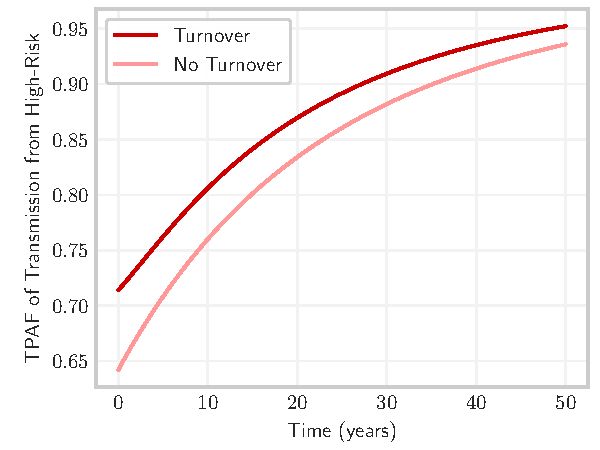
\includegraphics[width=0.45\linewidth]{sit-tpaf-tpaf-high-all-vs=fit}
  \caption{Transmission population attributable fraction (TPAF-from)
    of the high risk group in models with and without turnover,
    after fitting contact rates to group-specific prevalence.}
  \label{fig:tpaf-fit}
\end{figure}
% LW: I think this is the key message and valid.
% SS: This section perhaps could be a bit clearer as clearly very important
%     Is there a way to more explicitly talk about new infections
%     in the low / medium risks coming from prevalent infections
%     entering into these states from high risk groups and that
%     subsequent infections emanating from these individuals are thus still
%     linked back to prior history in the high risk group?
% JK: Great point and I realized this was not emphasized anywhere in the paper.
%     However, I think this section is not the right place for it,
%     as the increase in TPAF is really attributable to the higher estimated
%     contact rate ratio from Experiment 2.
%     However, I highlight that infections in low risk groups can originate
%     from higher risk period in the discussion,
%     since it kind of gets lost in Experiment 1.